\section{Implementation}
\subsection{RPC Server Design}
\begin{frame}
  \frametitle{RPC Server Design}
  We implement all the components in our system as RPC servers.
  \begin{itemize}
    \item Lowers coupling between components.
    \item Enables changing configurations or upgrading the system
      without halting the system.
    \item Roystonea\footnote[frame]{\tiny\fullcite{cite:roystonea}}
      benefits from this design, too.
  \end{itemize}
\end{frame}
\subsection{Task Queuing}
\begin{frame}
  \frametitle{Task Queuing}
  \begin{itemize}
    \item Workers are occupied until all tasks of the assigned job are
      done.
    \item Trailing idle workers.
    \item Maintain a available worker queue for each job.
    \item Enables releasing trailing idle workers earlier.
  \end{itemize}
\end{frame}

\begin{frame}
  \frametitle{Trailing Idle Worker}

  \begin{figure}[h]
    \centering
    \resizebox{\textheight}{!}{
      \pgfdeclarelayer{background}
\pgfsetlayers{background,main}
\begin{tikzpicture}
  \matrix (wmtrx2)[worker-matrix]{
    \node(w0_)[fill=red!15]{$w_0$};& \node(i1)[invisible]{};& \node(w0_)[fill=red!15]{$w_0$};&	\node(j1)[invisible]{};&	\node(w0_)[fill=red!15]{$w_0$};\\
    \node(w1_)[fill=red!15]{$w_1$};& \node(i2)[invisible]{};& \node(w1_)[fill=red!15]{$w_1$};&	\node(j2)[invisible]{};&	\node(w1_)[fill=red!15]{$w_1$};\\
    \node(w2_)[fill=red!15]{$w_2$};& \node(i3)[invisible]{};& \node(w2_)[fill=red!15]{$w_2$};&	\node(j3)[invisible]{};&	\node(w2_){$w_2$};\\
    \node(w3_)[fill=red!15]{$w_3$};& \node(i4)[invisible]{};& \node(w3_)[fill=red!15]{$w_3$};&	\node(j4)[invisible]{};&	\node(w3_){$w_3$};\\
  };
  \node[fit=(i1) (i4)]{};
  \node[fit=(j1) (j4)]{};
\end{tikzpicture}

    }
    \caption{Trailing Idle Worker}
  \end{figure}
\end{frame}

\subsection{Adaptive Adjustment}
\begin{frame}
  \frametitle{Adaptive Adjustment}
  \setbeamercovered{transparent}
  \only<1-5>{
    \begin{itemize}[<+->]
      \item We assumed that the execution time of each task can be
        predicted or obtained by profiling.
      \item <.->But accurate information is not always available.
        \begin{itemize}
          \item New applications
          \item Profiling error
          \item Machine performance degradation
        \end{itemize}
      \item Log the execution progress of each task and use it to
        estimate task execution speed
    \end{itemize}
  }
  \only<6>{
    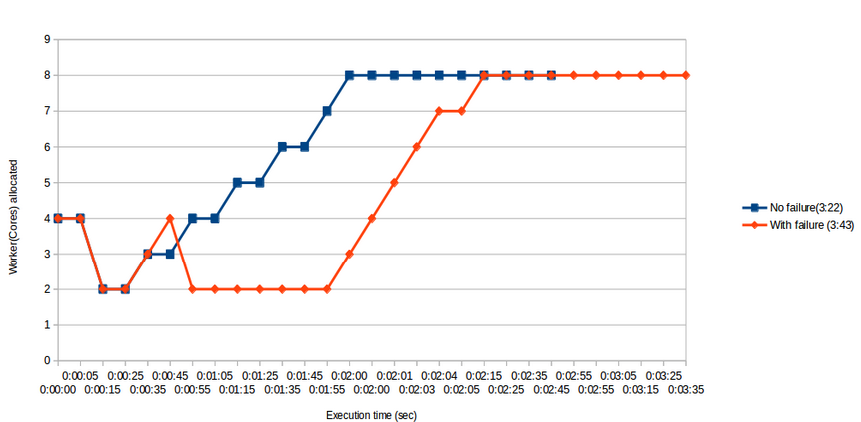
\includegraphics[width=\textwidth]{figures/adaptive.png}
  }
\end{frame}

\subsection{Case Study: Integration with JPPF}
\begin{frame}
  \frametitle{Case Study: Integration with JPPF}
  \only<1>{
    \begin{itemize}
      \item JPPF\footnote[frame]{\tiny\fullcite{cite:JPPF}} is a very
        popular open-source cluster management framework.
        \begin{itemize}
          \item Very easy to deploy
          \item GUI monitoring tools
          \item Active development
        \end{itemize}
      \item Used in CHT's cluster.
      \item Doesn't support \emph{centralized} and
        \emph{node-aware} scheduling
    \end{itemize}
  }
  \only<2->{
    \begin{itemize}[<+->]
      \item Provides API for jobs set "filters" for a job --- to reject a
        node from running that job
      \item<.-> Leveraging this API, we can somehow implement node-aware
        scheduling by
        \pause
        \begin{enumerate}
          \item Contact the system for scheduling information
          \item Get scheduled worker of the job
          \item Reject if this node is not scheduled
        \end{enumerate}
    \end{itemize}
  }
\end{frame}
